\documentclass[9pt, aspectratio=169]{beamer}
\usepackage{FiraSans}
\usetheme[subsectionpage=progressbar]{metropolis}
\usepackage[utf8]{inputenc}
\usepackage{amsmath}
\usepackage{amsfonts}
\usepackage{amssymb}
\usepackage{multicol}
\usepackage{tikz}
\usepackage{caption}
\usepackage{xcolor}
\usepackage[T1]{fontenc} 
\usepackage[skins]{tcolorbox}
\author{Nicola Roman\`o - nicola.romano@ed.ac.uk}
\title{Lecture 06 - Segmentation}
\setlength{\fboxsep}{0pt}
\setbeamertemplate {footline}{\begin{scriptsize}\hfill\insertframenumber ~of \inserttotalframenumber\kern1em\vskip5pt\end{scriptsize}}

% Remove "Figure" in front of captions
% See https://tex.stackexchange.com/questions/82456/how-to-remove-figure-caption-prefix-figure-in-beamer
\captionsetup{labelformat=empty,labelsep=none}

\titlegraphic{\centering 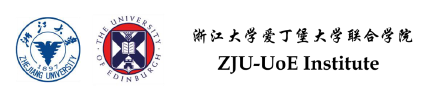
\includegraphics[scale=.5]{instituteLogo.png}}
\date{}

\begin{document}

\newtcolorbox{codebox}{enhanced,
    top=2pt,
    left=2pt,
    right=2pt,
    bottom=2pt,
    boxrule=0pt,
    leftrule=5pt,
    sharp corners,
    colback=gray!20,
    colframe=blue!60!black}

\begin{frame}
    \titlepage
\end{frame}

\begin{frame}
    {Learning objectives}
    \begin{columns}
        \begin{column}{0.8\textwidth}
            \begin{itemize}
                \item LO 1
                \item LO 2
                \item LO 3
            \end{itemize}
        \end{column}
        \begin{column}{0.2\textwidth}
            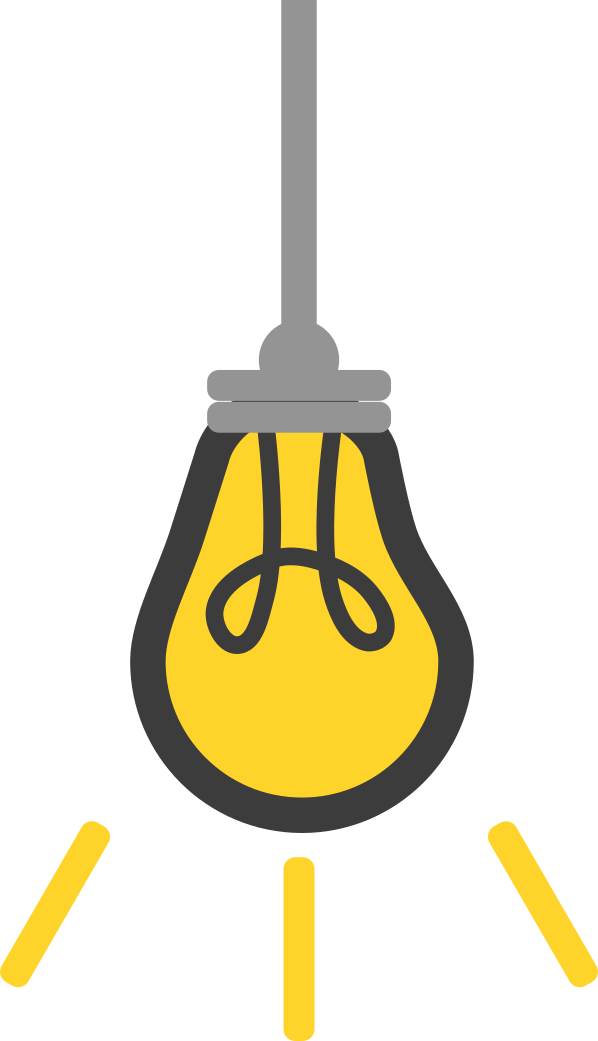
\includegraphics[angle=-30, origin=tr, width=1.5\textwidth]{lightbulb.png}
        \end{column}
    \end{columns}
\end{frame}

\section{Introduction}

\begin{frame}
    {Segmentation - definition}
    \begin{itemize}
        \item Segmentation is a long-studied (and complex!) problem in computer vision.
        \item Process of dividing an image into sets of pixels called \textit{segments} or \textit{objects}
        \item Each pixel gets a label identifying which object it belongs to.
        \item The different segments can then be analysed independently.
    \end{itemize}
\end{frame}

\begin{frame}
    {Application of segmentation}
    In biomedical imaging
    \begin{itemize}
        \item Segmentation of cells to measure their properties
        \item Analysis of X-ray images to identify pathologies
        \item Aid in surgery planning
    \end{itemize}
    \pause
    In computer vision in general
    \begin{itemize}
        \item Car, pedestrian, break lights detection (e.g. for autonomous car navigation)
        \item Face detection (e.g. for facial recognition, emotion analysis etc.)
        \item Fingerprint recognition
        \item \dots
    \end{itemize}
\end{frame}

\begin{frame}
    {Methods for segmentation}
    Segmentation is a difficult problem to solve, with many important practical applications, so it has been widely studied.

    \pause

    This lecture will cover some of the \textbf{traditional methods} for image segmentation. More recent \textbf{machine learning-based methods} will be covered later in the course.
\end{frame}

\begin{frame}
    {Semantic segmentation vs instance segmentation}
    There are two main types of segmentation:

    \begin{itemize}
        \item \textbf{Semantic segmentation}: divides the image in regions, each of which belongs to a specific class. Multiple objects of the same class will be detected in the same region.
        \item \textbf{Instance segmentation}: divides the image in regions, each of which is an instance of a class. Multiple objects of the same class will be detected as separate regions.
    \end{itemize}
\end{frame}

\begin{frame}
    {Semantic segmentation vs instance segmentation - an example}
    \only<1>{
        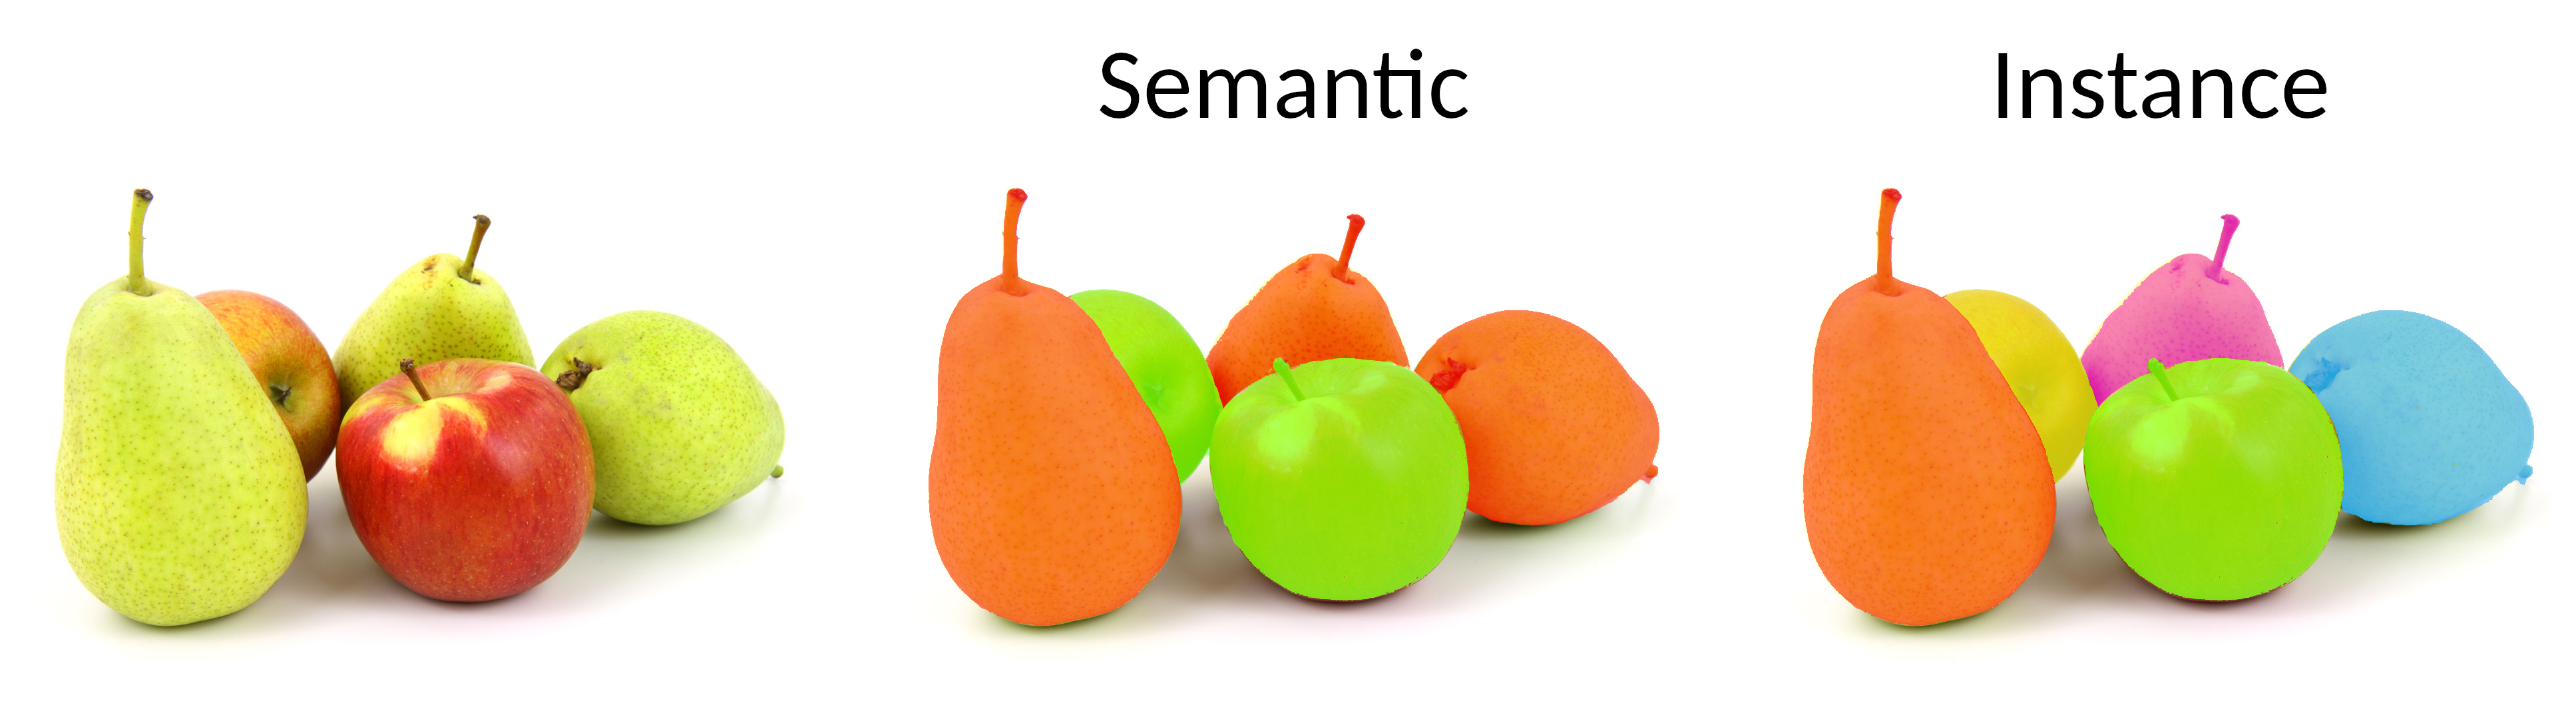
\includegraphics[width=\textwidth]{semantic_vs_instance_cv.jpg}
        \footnotesize
        Source: Apples and pears - Petr Kratochvil - CC0
    }
    \only<2>{
        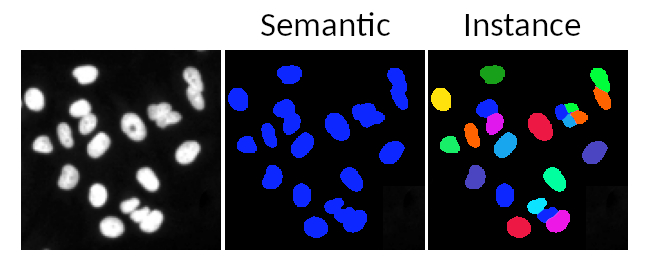
\includegraphics[width=\textwidth]{semantic_vs_instance_bio.jpg}
        \footnotesize
        Source: Nicola Roman\`o
    }
\end{frame}

\section{Semantic segmentation - thresholding methods}

\begin{frame}
    {Thresholding}
    Thresholding is the simplest way of performing semantic segmentation, when there is a clear distinction between the object(s) of interest and the background.

    We define a threshold $t$ and create a mask $M$ such that:

    $$M(x, y) = \begin{cases}
            0 & \text{for}~I(x,y) < t    \\
            1 & \text{for}~I(x,y) \geq t \\
        \end{cases}$$

    \pause
    This can be extended to multi-class segmentation by chosing $t_1, t_2, \dots, t_n$ and generating a mask

    $$M(x, y) = \begin{cases}
            0 & \text{for}~I(x,y) < t_1          \\
            1 & \text{for}~t_1 \leq I(x,y) < t_2 \\
            \dots                                \\
            n & \text{for}~I(x,y) > t_n          \\
        \end{cases}$$
\end{frame}

\begin{frame}
    {Choosing a threshold}
    We can manually choose a threshold by inspecting the image histogram

    \centering
    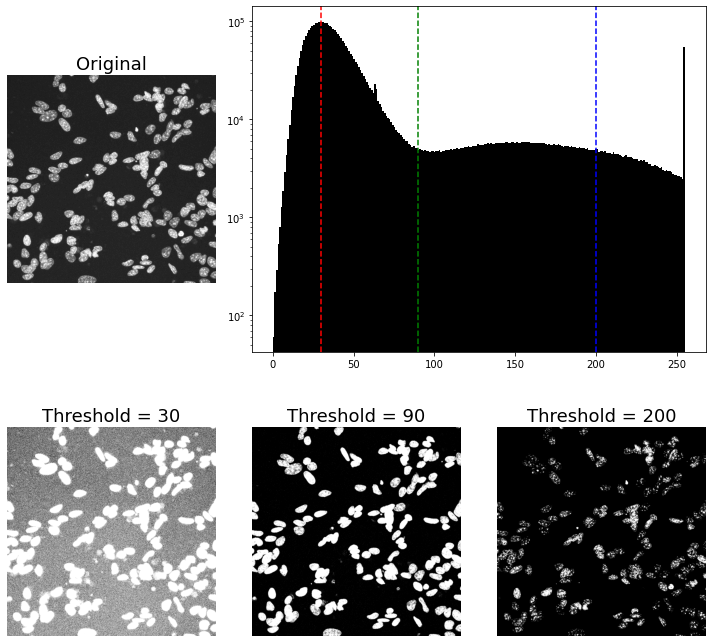
\includegraphics[height=.75\textheight]{manual_thresholding.png}

    \pause
    \textbf{Is there a better way?}
\end{frame}

\begin{frame}
    {Otsu's method}
    Otsu's method is a simple way to automatically choose a threshold.

    The algorithm makes an exhaustive search for the optimal threshold that maximizes the between-class variance (equivalent to minimizing the intra-class variance).

    \large
    $$\sigma_\omega^2 = \omega_0\sigma_0^2+\omega_1\sigma_1^2$$
    $$\omega_0 =\sum_{i=0}^{t-1} p(i)\qquad\omega_1 =\sum_{i=t}^{L-1} p(i)$$
\end{frame}

\begin{frame}
    {Otsu's method - an example}
    \begin{columns}
        \begin{column}{.6\textwidth}
            \begin{codebox}
                \texttt{from skimage.filters import threshold\_otsu\\
                    \\
                    t = threshold\_otsu(img)\\
                    \\
                    plt.imshow(img > t, cmap="gray")\\
                    plt.axis("off")\\
                    plt.title(f"Otsu's threshold (\{t\})", fontsize=18)\\
                    plt.show()}
            \end{codebox}
        \end{column}
        \begin{column}{.4\textwidth}
            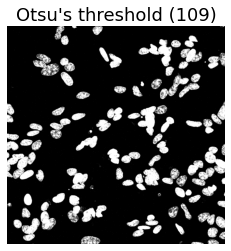
\includegraphics[width=\textwidth]{otsu's threshold.png}
        \end{column}
    \end{columns}
\end{frame}

\begin{frame}
{Issues with thresholding}

\begin{itemize}
    \item Noise is a problem -> Gaussian (or median) filter helps
    \item Need to remove holes afterwards
\end{itemize}
\centering
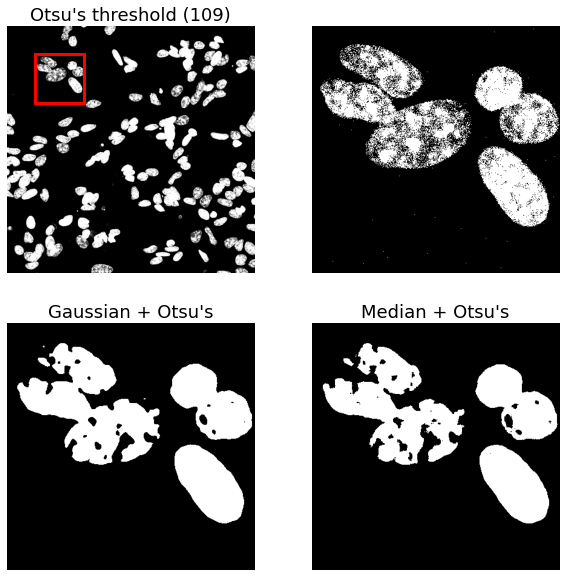
\includegraphics[width=.4\textwidth]{otsu_and_smoothing.png}
\end{frame}

\begin{frame}
{Filling holes}
Morphological operations allow to fill small holes. 
The `skimage.morphology.remove\_small\_holes` function is an example of such an operation.

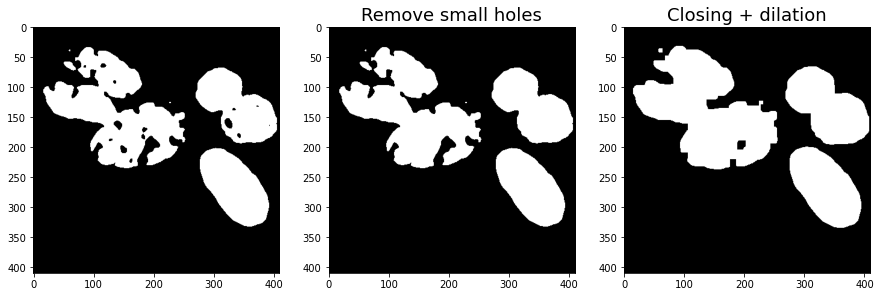
\includegraphics[width=\textwidth]{morphological.png}
\end{frame}
\begin{frame}
    {Multi-Otsu segmentation}
    The Otsu's method can be extended to multi-class segmentation.

    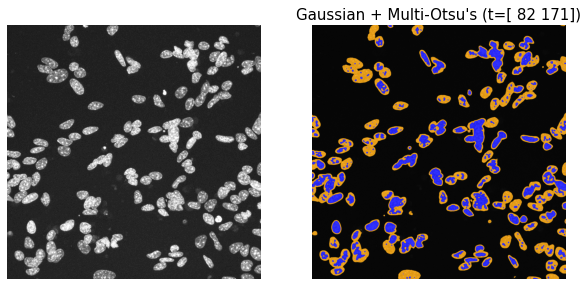
\includegraphics[width=\textwidth]{multiotsu.png}
\end{frame}

\begin{frame}
{Multi-Otsu segmentation - code}
\begin{codebox}
\texttt{from skimage.filters import threshold\_multiotsu, gaussian\\
from skimage import img\_as\_ubyte\\
import numpy as np\\
from skimage.color import label2rgb\\
\\
t = threshold\_multiotsu(img, classes=3)\\
\\
\# Remember to go back to unsigned 8-bit integers from float!\\
img\_gaus = img\_as\_ubyte(gaussian(img, 5))\\
\# Convert to mask with 3 levels\\
img\_thr\_gaus = np.digitize(img\_gaus, t)\\
\\
\# Handy function to map the labels to colors\\
img\_with\_overlay = label2rgb(img\_thr\_gaus, image = img, bg\_label=0, colors = ["orange", "blue"], alpha = .8)\\
\\
\# Then visualise using Matplotlib!
\\
}
\end{codebox}
\end{frame}

\section{Clustering methods}

\begin{frame}
{K-means segmentation}
\end{frame}

\begin{frame}
{Voronoi segmentation}
\end{frame}
\section{Instance segmentation}
\subsection{Watershed}

\begin{frame}
{Watershed}

\end{frame}
\end{document}

